\documentclass{beamer}
\useoutertheme[subsection=false]{miniframes}

\usepackage[style=authoryear, sorting=none]{biblatex}
\addbibresource{bibliography.bib}

\title{Does Crime Pay? Co-Evolution of Insider Trading and its Regulation}
\author{Jagdev Bal, Ellie Fadipe, Jade Jones, Alex Room}
\date{4th of May, 2023}

\begin{document}
\begin{frame}
\titlepage
\end{frame}


\section{Introduction}
% Introduce insider trading
\begin{frame}{Introduction}
\begin{itemize}
    \item What is insider trading?
    \item How does it appear in markets?
\end{itemize}
\end{frame}

% Introduce our investigation
\begin{frame}{Introduction}
    
\end{frame}


\section{Methods}
% Introduce notation and game model
\begin{frame}{Stage Game}
Players are a trader, $\mathcal{T}$, and regulator, $\mathcal{R}$, with actions:
\begin{itemize}
\item $\mathcal{A}_\mathcal{T}$ = \{\text{regular trade}, \text{inside trade}\}
\item $\mathcal{A}_\mathcal{R}$ = \{\text{no investigation}, \text{investigation}\}
\end{itemize}

and payoff matrices:
\begin{equation*}
\begin{split}
    \mathcal{T}: 
    \begin{pmatrix}
    1 & 1 \\
    6 & -10
    \end{pmatrix}
\end{split}
\quad\quad
\begin{split}
    \mathcal{R}: 
    \begin{pmatrix}
    1 & -1 \\
    -3 & 5
    \end{pmatrix}
\end{split}
\end{equation*}

\end{frame}

% describe information and strategies
\begin{frame}{Information}
\begin{figure}
\centering
\begin{tabular}{c c}
Prisoner's Dilemma & Our Model \\
\begin{tabular}{p{0.2\textwidth} p{0.2\textwidth}}
Player 1 & Player 2 \\
\hline\hline
Full information & Full information
\end{tabular} &

\begin{tabular}{p{0.2\textwidth} p{0.2\textwidth}}
Player 1 ($\mathcal{T}$) & Player 2 ($\mathcal{R}$)\\
\hline\hline
Full information & Can't identify all defection
\end{tabular}
\end{tabular}
\end{figure}
\end{frame}

\begin{frame}{Traders}
\begin{figure}
\centering
\begin{tabular}{l l l}
Name & Properties \\
\hline\hline
\texttt{Cooperator} & Cooperative, Unresponsive \\
\texttt{CoastClear} & Exploitative, Responsive \\
\texttt{NceBitten:5} & Exploitative, Partially Responsive \\
\texttt{Careful} & Risk-Averse, Responsive \\
\texttt{Random:0.8} & Risk-Averse, Unresponsive \\
\texttt{Tit for Two Tats} & Risk-Averse, Responsive \\
\end{tabular}
\end{figure}
\end{frame}

\begin{frame}{Regulators}
\begin{figure}
\centering
\begin{tabular}{l l l}
Name & Properties \\
\hline\hline
\texttt{SuspiciousGrudge} & Responsive, Unforgiving \\
\texttt{SuspiciousForgiving} & Responsive, Forgiving \\
\texttt{Grudge} & Unforgiving, Partially Responsive \\
\texttt{Random:0.2} & Random, Unresponsive \\
\texttt{BudgetStretcher} & Risk-Averse, Responsive \\
\end{tabular}
\end{figure}
\end{frame}


% describe the paired Moran process
\begin{frame}{Paired Moran Process\footnote{cf. \fullcite{shakarian2013novel}}}
\begin{itemize}
\item We take two populations, $P_1$, $P_2$, of row and column players respectively
\item The fitness functions are 'paired' between the populations
\item But birth and death is independent!
\end{itemize}
\end{frame}

\begin{frame}{Why?}
\begin{itemize}
    \item Information sets are uneven
    \item Populations don't interact within themselves
    \item Populations don't have utilities on the same "scale"
    \item Strategies don't 'carry over'
\end{itemize}
\end{frame}


\section{Results}
% co-winners heatmap
\begin{frame}{Co-Winners}
\begin{figure}[!h]
    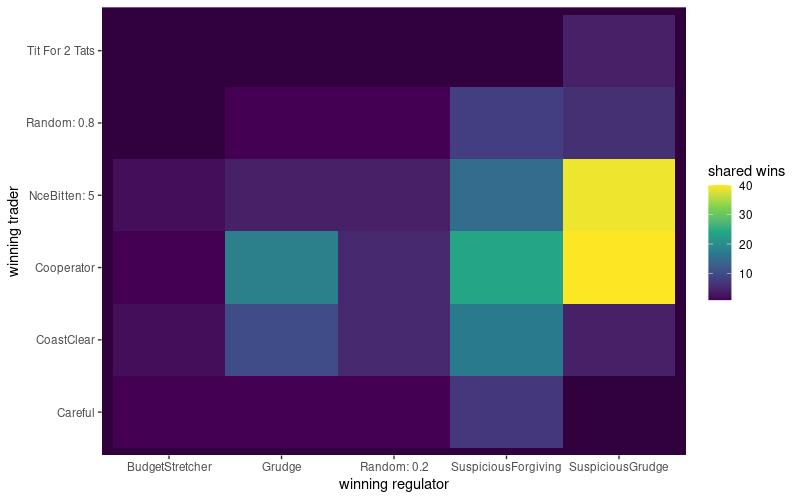
\includegraphics[width=\textwidth]{heatmap.png}
    \caption{A heatmap of co-winning trader-regulator pairs}
    \label{fig:f1}
\end{figure}
\end{frame}

% strategy survival for traders
\begin{frame}{Strategy Survival}
\begin{figure}[!h]
    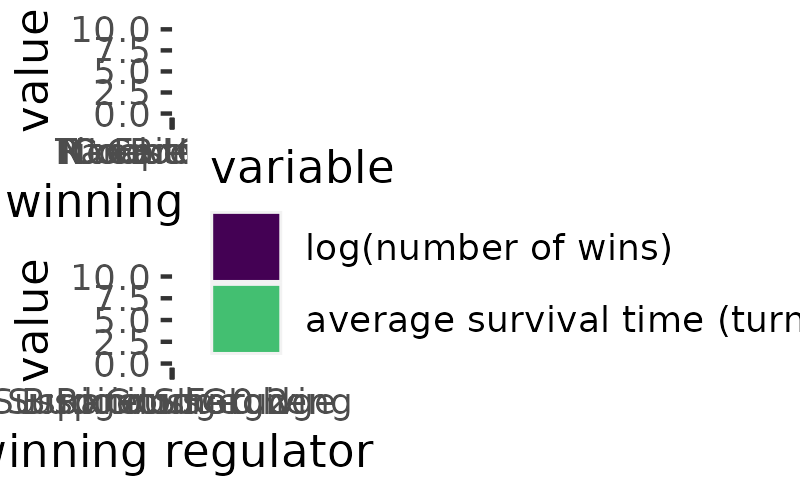
\includegraphics[width=\textwidth]{barplot.png}
    \caption{The number of wins (log base 10) and average survival time (in turns) of each trader/regulator}
    \label{fig:f2}
\end{figure}

\end{frame}

% strategy survival for regulators
\begin{frame}{Strategy Survival}
    
\end{frame}


\section{Conclusions}
% conclusions on data
\begin{frame}{Conclusions: Data}
\begin{itemize}
    \item Cooperation or "strategic exploitation"\footnote{\fullcite{kyle1985continuous}}
    \item 
    \item Further study into strength of punishment and its effects on the market\footnote{\fullcite{smales2017game}}
\end{itemize}
\end{frame}

% conclusions on algorithms
\begin{frame}{Conclusions: Algorithm}

\end{frame}



\end{document}
